\chapter{Descrizione del Progetto}
\label{cap:descrizione}
Questo capitolo introduce i preliminari tecnici e illustra il problema affrontato. La sezione \ref{Scenario} è dedicata alla descrizione del contesto tecnologico mentre la sezione \ref{Problema} analizza le problematiche affrontate nello studio. 

\section{Scenario Tecnico}
\label{Scenario}

\subsection{Malware}
Il termine "malware" deriva dall'unione delle parole inglesi \emph{malicious} e \emph{software}\cite{site:malware} e indica qualsiasi programma o codice progettato per infiltrarsi, danneggiare o ottenere l'accesso non autorizzato a un sistema informatico. I malware possono essere creati con diversi scopi, come il furto di informazioni sensibili, il sabotaggio di sistemi, la visualizzazione di pubblicità indesiderata, o il ricatto delle vittime. Esistono varie tipologie di malware, ognuna con specifiche caratteristiche e metodi di azione.

\subsubsection{Famiglie di Malware}
Esistono molte famiglie di malware, ognuna con caratteristiche particolari e comportamenti distinti. Tra le più conosciute, possiamo citare:
\begin{itemize}
    \item \textbf{Adware}: Nasce dall'unione di \emph{advertising} e \emph{software} ed è un'applicazione software in cui un banner pubblicitario o altro materiale pubblicitario vengono visualizzati e scaricati mentre un programma è in esecuzione.
    L'adware legittimo viene scaricato con il consenso esplicito degli utenti. Questi ultimi scaricano consapevolmente questa forma di adware e di solito ottengono qualcosa in cambio. Potrebbero ottenere uno sconto o software gratuito in cambio della ricezione dell'adware. Gli annunci aiutano a coprire i costi di sviluppo del software o consentono allo sviluppatore di fornire il prodotto gratuitamente.
    L'adware è malevolo quando viene progettato con l'intento di fornire software dannoso all'utente. Il software viene classificato come spyware se viene eseguito all'insaputa e senza l'autorizzazione dell'utente. I dati degli utenti raccolti in questo modo vengono spesso venduti a terzi.
    \item \textbf{Backdoor}: Un tipo di malware che consente l'accesso remoto non autorizzato a un sistema, permettendo all'attaccante di controllare il dispositivo senza che l'utente ne sia a conoscenza. Tra i potenziali rischi vi è l'installazione di keylogger nel computer, strumenti che registrano ogni tasto premuto, consentendo ai malintenzionati di sottrarre dati sensibili come le password degli account.
    \item \textbf{Downloader}: Malware progettato per scaricare e installare altri malware su un dispositivo infetto. Spesso funge da primo stadio di un'infezione più complessa, preparando il terreno per l'installazione di altri malware come trojan, ransomware o spyware.
    \item \textbf{Ransomware}: Malware progettato per criptare i dati dell'utente e richiedere un riscatto per la decrittazione. Spesso utilizza tecniche di estorsione per costringere le vittime a pagare somme di denaro in criptovalute.
    \item \textbf{Spyware}: Malware progettato per raccogliere informazioni sull'utente senza il suo consenso, come dati personali, cronologia di navigazione e credenziali, per poi inviarle all'attaccante.
    \item \textbf{Trojan (Cavalli di Troia)}: Programmi che si mascherano come software legittimi per ingannare gli utenti e indurli a installarli. Una volta installati, possono dare accesso al sistema o danneggiarlo.
    \item \textbf{Virus}: Software che si replica infettando altri file eseguibili, spesso con l'intento di danneggiare il sistema o rubare informazioni.
    \item \textbf{Worms}: Simili ai virus, ma non necessitano di un file host per propagarsi. Possono diffondersi autonomamente attraverso la rete, sfruttando vulnerabilità di sicurezza.
    \item \textbf{Rootkit}: Malware progettato per nascondere la presenza di altri malware o del proprio codice su un sistema, integrandosi profondamente nel sistema operativo e rendendosi quasi invisibile agli strumenti di rilevamento tradizionali.
    \item \textbf{Keylogger}: Un tipo di malware che registra ogni battitura dell'utente su tastiera per rubare informazioni sensibili come password e credenziali di accesso.
    \item \textbf{Botnet}: Una rete di dispositivi infetti che possono essere controllati a distanza per compiere azioni malevole, come attacchi DDoS e spam.
    \item \textbf{Fileless Malware}: Malware che non scrive alcun file sul disco, utilizzando invece la memoria e strumenti già esistenti nel sistema operativo, rendendo più difficile la rilevazione.
    \item \textbf{Scareware}: Malware che inganna l'utente facendogli credere che il sistema sia infettato per indurlo a comprare software falsi o fornire informazioni personali.
    \item \textbf{RAT (Remote Access Trojan)}: Trojan che permette all'attaccante di ottenere accesso remoto e controllo completo del dispositivo infetto, consentendo di spiare l'utente e rubare informazioni.
    \item \textbf{Malvertising}: Uso di annunci pubblicitari legittimi per distribuire malware, spesso sfruttando reti pubblicitarie per diffondere link malevoli.
    \item \textbf{Cryptojacker}: Malware che utilizza le risorse di calcolo della vittima per effettuare il mining di criptovalute senza che l'utente ne sia consapevole.
    \item \textbf{Logic Bomb}: Malware che rimane inattivo fino a quando non viene attivato da un evento specifico, come una data o una certa condizione, per poi eseguire azioni malevole come cancellare file o causare crash del sistema.
\end{itemize}

\subsubsection{Struttura del malware}
La struttura tipica di un malware varia in base alla tipologia di famiglia a cui il malware appartiene, le più comuni sono:
\begin{itemize}
    \item \textbf{Adware}: Include componenti per il monitoraggio delle abitudini di navigazione dell'utente, e un motore per la visualizzazione automatica di annunci pubblicitari.
    \item \textbf{Backdoor}: Contiene un modulo che consente l'accesso remoto non autorizzato, spesso implementato tramite una comunicazione criptata con il server di controllo dell'attaccante.
    \item \textbf{Downloader}: Dispone di un componente per contattare server remoti e scaricare ulteriori malware, spesso utilizzando tecniche di offuscamento per eludere la rilevazione.
    \item \textbf{Ransomware}: Presenta un sistema di criptazione che rende inaccessibili i dati dell'utente, accompagnato da un modulo che mostra un messaggio di riscatto e gestisce i pagamenti.
    \item \textbf{Spyware}: Ha moduli per il keylogging, il monitoraggio della cronologia di navigazione e la raccolta di credenziali, inviando poi queste informazioni agli attaccanti.
    \item \textbf{Trojan}: Include un componente di mimetizzazione, spesso mascherandosi da software legittimo, e può implementare diversi payload per danneggiare il sistema o esfiltrare dati.
    \item \textbf{Virus}: Contiene un modulo di replicazione che gli consente di infettare altri file eseguibili, spesso con funzionalità aggiuntive per danneggiare il sistema.
    \item \textbf{Worms}: Dispone di un motore di propagazione automatica, che sfrutta vulnerabilità note per diffondersi in modo autonomo tra i dispositivi connessi in rete.
    \item \textbf{Rootkit}: Include un modulo per nascondere la presenza del malware all'interno del sistema, modificando componenti del kernel o altri elementi critici del sistema operativo.
    \item \textbf{Keylogger}: Dispone di un modulo per catturare tutte le battiture dell'utente, salvandole in un file log da inviare all'attaccante.
    \item \textbf{Botnet}: Include componenti che consentono di trasformare il dispositivo in un "bot" controllato da remoto, spesso senza che l'utente ne sia consapevole.
    \item \textbf{Fileless Malware}: Utilizza strumenti nativi del sistema operativo (come PowerShell o WMI) per eseguire codice dannoso direttamente in memoria, rendendo più difficile la sua rilevazione.
    \item \textbf{Scareware}: Contiene un modulo per la visualizzazione di avvisi falsi che spingono l'utente ad acquistare software non necessario o dannoso.
    \item \textbf{RAT (Remote Access Trojan)}: Include strumenti per il controllo remoto, consentendo all'attaccante di navigare tra i file, attivare la webcam e installare altri malware.
    \item \textbf{Malvertising}: Contiene codice che viene iniettato tramite banner pubblicitari, spesso sfruttando vulnerabilità del browser per compromettere il sistema dell'utente.
    \item \textbf{Cryptojacker}: Include script di mining che si attivano all'insaputa dell'utente per utilizzare risorse di CPU e GPU per minare criptovalute.
    \item \textbf{Logic Bomb}: Include una condizione preimpostata (come una data specifica o un certo evento) che, una volta soddisfatta, attiva il payload dannoso.
\end{itemize}

\subsubsection{Dataset}
Nell'ambito di questo progetto di ricerca sono state prese in considerazione solo le prime sette famiglie di malware, in quanto le più comuni e pericolose. Per la raccolta del dataset sono stati utilizzati campioni di malware provenienti da diverse fonti, tra cui:
\begin{itemize}
    \item \textbf{MalwareBazaar}: Una piattaforma gestita da abuse.ch e Spamhaus, dedicata alla condivisione di campioni di malware con la comunità di sicurezza informatica, fornitori di antivirus e provider di intelligence sulle minacce. Gli utenti possono caricare campioni di malware e esplorare il database per ottenere informazioni preziose. La piattaforma offre anche API per integrare i dati nei sistemi di gestione delle informazioni e degli eventi di sicurezza (SIEM) o in altre piattaforme di intelligence sulle minacce.
    \item \textbf{MalShare}: Un progetto comunitario che offre un repository pubblico di malware, fornendo accesso gratuito a campioni di malware e strumenti alla comunità di sicurezza informatica. Gli utenti possono cercare campioni utilizzando hash, nomi di file, nomi di regole Yara o fonti. La piattaforma è progettata per facilitare la condivisione e l'analisi dei campioni di malware tra i professionisti della sicurezza.
    \item \textbf{VirusShare}: Una piattaforma che fornisce accesso a un ampio repository di campioni di malware. È utilizzata da ricercatori di sicurezza informatica, analisti e organizzazioni per ottenere campioni da analizzare e studiare il comportamento del malware. La piattaforma è guidata dalla comunità, con campioni contribuiti da ricercatori e professionisti della sicurezza informatica di tutto il mondo.
\end{itemize}

Per la classificazione dei campioni di malware sono stati utilizzati diversi strumenti di analisi statica e dinamica, tra cui:
\begin{itemize}
    \item \textbf{Virustotal}: Un servizio online che consente l'analisi di file e URL sospetti per identificare malware e altri tipi di contenuti dannosi. Fondato nel 2004 e acquisito da Google nel 2012, VirusTotal aggrega i risultati di oltre 70 motori antivirus e strumenti di scansione URL, offrendo una panoramica completa sulla sicurezza di un file o di un sito web. Gli utenti possono caricare file o inserire URL per ottenere un rapporto dettagliato che indica quali motori hanno rilevato minacce e quali no. VirusTotal fornisce anche API per l'integrazione con altri strumenti e servizi di sicurezza.
    \item \textbf{AVClass2}: Uno strumento automatico per l'estrazione di tag da etichette antivirus (AV), progettato per categorizzare campioni di malware su larga scala. Sviluppato per migliorare le capacità del suo predecessore, AVClass, AVClass2 non si limita a identificare solo i nomi delle famiglie di malware, ma estrae anche informazioni su classi di malware, comportamenti e proprietà dei file. Utilizza e contribuisce a costruire una tassonomia aperta che organizza i concetti presenti nelle etichette AV, permettendo di gestire nuovi tag introdotti dai fornitori di antivirus nel tempo.
    \item \textbf{Ghidra}: Una suite di strumenti per l'ingegneria inversa di software, sviluppata dalla National Security Agency (NSA) degli Stati Uniti e resa disponibile al pubblico nel 2019. Questa piattaforma open-source consente agli analisti di sicurezza di decompilare, disassemblare e analizzare binari compilati, facilitando la comprensione del funzionamento interno di software sospetti o malevoli. Ghidra supporta una vasta gamma di architetture e formati di file, offrendo funzionalità avanzate come un potente decompilatore e un'interfaccia utente grafica intuitiva.
\end{itemize}

\vspace{.5cm}
Il dataset risultante è composto come segue:
\begin{table}[h]
    \centering
    \begin{tabular}{|l|c|}
        \hline
        \textbf{Famiglia di Malware} & \textbf{Numero di Campioni} \\
        \hline
        Adware & 4566 \\
        \hline
        Backdoor & 1270 \\
        \hline
        Downloader & 1128 \\
        \hline
        Ransomware & 2529 \\
        \hline
        Spyware & 502 \\
        \hline
        Trojan & 4058 \\
        \hline
        Virus & 2061 \\
        \hline
    \end{tabular}
    \vspace{.2cm}
    \caption{\emph{Dataset di malware impiegato nel progetto di ricerca}}
\end{table}

\begin{figure}
    \centering
    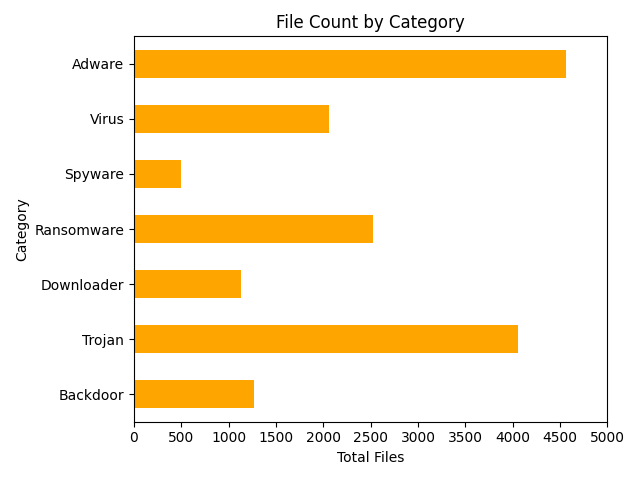
\includegraphics[width=0.7\textwidth]{images/total_families.png}
    \caption{\emph{Famiglie di malware presenti nel dataset del progetto di ricerca}}
\end{figure}

\newpage

\subsection{Decompilatore}
Nonostante siano disponibili numerose tipologie di decompilatori, in questo progetto si è scelto l'utilizzo di \textbf{Ghidra} in quanto open source, già utilizzato in precedenza e compatibile con architettura arm presente nella macchina utilizzata durante tutto il tempo di svolgimento del progetto. È uno strumento di analisi di software, principalmente noto come un potente decompilatore e framework per il \gls{reverseengineering}, sviluppato e distribuito gratuitamente dalla National Security Agency (NSA) degli Stati Uniti. Il suo utilizzo in questo progetto consiste in:
\begin{itemize}
    \item Decompilazione del codice eseguibile in \textbf{codice assembly} su cui poter effettuare analisi statica in un secondo momento. 
    \item Estrazione del \textbf{codice esadecimale}, facilitando ulteriori esami e manipolazioni del codice.
\end{itemize}

\subsection{Convolutional Neural Network}
Per l'addestramento di questa rete neurale è stato adottato Keras\cite{site:keras} con TensorFlow\cite{site:tensorflow}, una libreria open-source per il machine learning e il deep learning.
L'architettura della rete neurale convoluzionale (CNN) utilizzata in questo progetto è composta da diversi strati, ciascuno con un ruolo specifico nel processo di apprendimento:
\begin{enumerate}
    \item \textbf{Strati Convoluzionali (Conv2D)}:
    La rete inizia con tre strati convoluzionali, che sono responsabili dell'estrazione delle caratteristiche principali dalle immagini di input in scala di grigi (16x16 pixel).
    Primo strato convoluzionale: utilizza da 32 a 128 filtri (incremento di 32) con kernel di dimensione (3x3). Questo strato mantiene l'input della stessa dimensione (16x16) grazie al padding "same" e utilizza l'attivazione ReLU (Rectified Linear Unit).
    Secondo strato convoluzionale: utilizza da 32 a 64 filtri (incremento di 32) con kernel (3x3) e l'attivazione ReLU, seguito da un'operazione di MaxPooling2D con finestra (2x2), riducendo così la dimensione a (8x8).
    Terzo strato convoluzionale: impiega lo stesso numero di filtri (32-64, incremento di 32) e kernel, con un'ulteriore riduzione dimensionale tramite MaxPooling2D, portando la dimensione finale a (2x2).
    \item \textbf{Strato di Pooling (MaxPooling2D)}:
    Gli strati di pooling riducono la dimensione spaziale delle feature map mantenendo solo le informazioni più rilevanti, riducendo il numero di parametri e migliorando l'efficienza computazionale.
    Sono utilizzati dopo ogni strato convoluzionale con finestre di dimensione (2x2).
    \item \textbf{Strato di Flattening}:
    Dopo la fase convoluzionale, le feature map tridimensionali vengono "appiattite" in un vettore unidimensionale per poter essere processate dagli strati completamente connessi.
    \item \textbf{Strato Completamente Connesso (Dense)}:
    Lo strato completamente connesso riceve l'input dallo strato di flattening. Qui, i neuroni collegano ogni unità precedente a quelle successive, consentendo alla rete di apprendere pattern complessi e interazioni tra le caratteristiche estratte.
    La dimensione del layer è variabile tra 32 e 128 unità, con attivazione ReLU. È anche presente un layer di Dropout, utilizzato per prevenire l'\gls{overfitting} con un valore di \gls{dropout} che può variare tra 0.0 e 0.5 (incremento di 0.1).
    \item \textbf{Strato di Output (Dense)}:
    Lo strato finale è un layer completamente connesso con un numero di neuroni pari al numero di classi di malware presenti nel dataset, con attivazione Softmax per ottenere una probabilità normalizzata per ciascuna classe.
\end{enumerate}

\begin{figure}[ht]
    \centering
        \centering
        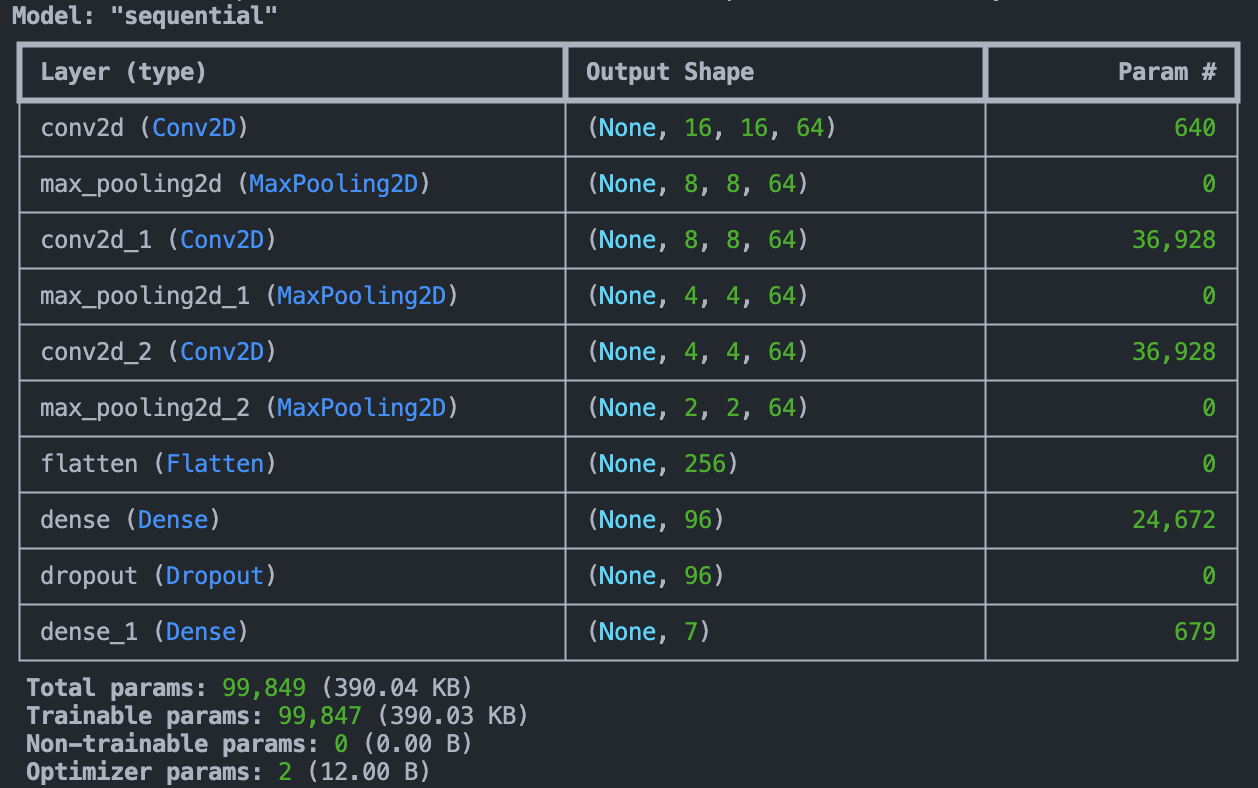
\includegraphics[width=0.8\linewidth]{images/cnn_architecture.png}
        \caption{\emph{Architettura della rete neurale convoluzionale (CNN) utilizzata}}
        \label{fig:cnn_architecture}
\end{figure}

\subsubsection{Processo di addestramento}
Per garantire un'efficace categorizzazione, il dataset è stato suddiviso in tre sottoinsiemi: 
\begin{itemize}
    \item \textbf{Training Set}: 80\% del dataset, utilizzato per addestrare il modello.
    \item \textbf{Validation Set}: 10\% del dataset, utilizzato per regolare i parametri del modello e prevenire l'overfitting.
    \item \textbf{Test Set}: 10\% del dataset, utilizzato per valutare le prestazioni del modello su dati non visti.
\end{itemize}
Il modello è stato progettato utilizzando una rete neurale convoluzionale (CNN), ottimizzata tramite Keras Tuner per la selezione automatica dei migliori \gls{hyperparameter}. L'ottimizzazione ha incluso la scelta del numero di filtri nelle convoluzioni, le unità dense e il tasso di dropout. Tra i parametri testati vi sono stati i filtri per i layer convoluzionali (con valori da 32 a 128), il numero di unità dense (tra 32 e 128) e il tasso di dropout (da 0,0 a 0,5).

Una volta identificata la configurazione ottimale, il modello è stato addestrato per 100 epoche utilizzando un \gls{batchsize} di 32, adottando l'algoritmo di ottimizzazione \gls{adam} e la funzione di perdita categorical\_crossentropy, adeguata per la classificazione multi\-classe. Durante l'addestramento, la validazione incrociata è stata impiegata per monitorare le prestazioni del modello sui dati di validazione.

Le prestazioni del modello sono state valutate sul dataset di test mediante metriche quali accuratezza, precisione, richiamo e F1-score, calcolate sia in media micro che macro. La \gls{confusionmatrix} è stata utilizzata per una visione dettagliata della capacità del modello di distinguere tra le diverse categorie di malware.

Per visualizzare l'efficacia dell'addestramento, sono stati generati grafici che mostrano l'andamento dell'accuratezza e della perdita sia per il training che per la validazione. Questi risultati sono stati salvati in formato grafico e i relativi valori metrici in file di testo, evidenziando le prestazioni complessive del modello.

\newpage
\begin{figure}[ht]
    \centering
        \centering
        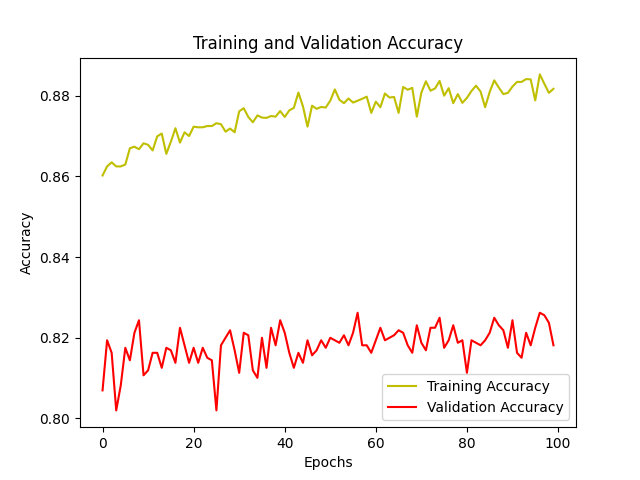
\includegraphics[width=0.7\linewidth]{images/cnn_accuracy.png}
        \label{fig:cnn_accuracy}
        \caption{\emph{Grafico dell'accuratezza del modello CNN durante l'addestramento e la validazione}}
\end{figure}

\begin{figure}[ht]
    \centering
        \centering
        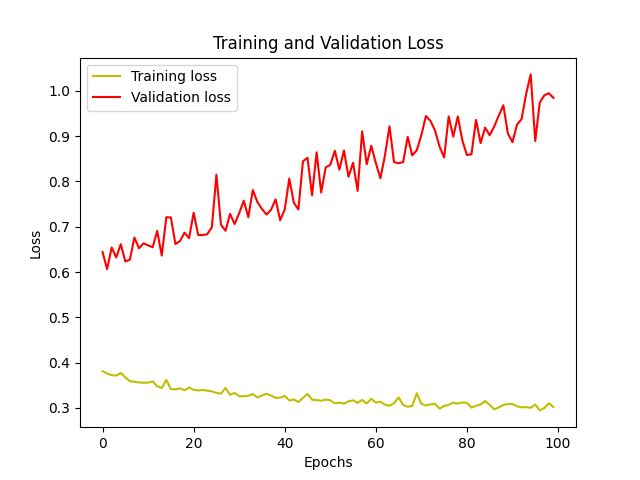
\includegraphics[width=0.7\linewidth]{images/cnn_loss.png}
        \label{fig:cnn_loss}
        \caption{\emph{Grafico della perdita del modello CNN durante l'addestramento e la validazione}}
\end{figure}

\newpage
\subsubsection{Metriche di Valutazione del Modello}
Nel campo della classificazione, specialmente in scenari complessi come la classificazione del malware, è importante analizzare le prestazioni del modello utilizzando diverse metriche. Ogni metrica offre una prospettiva unica sui punti di forza e debolezza del modello, fornendo una visione completa della sua capacità di generalizzare e discriminare tra le classi. Di seguito, una descrizione approfondita delle metriche adottate.

\subsubsubsection{Accuratezza}
L'accuratezza è la metrica più intuitiva e rappresenta la proporzione di predizioni corrette rispetto al totale delle predizioni effettuate. È calcolata come:
\[
\text{Accuratezza} = \frac{TP + TN}{TP + TN + FP + FN}
\]
In questo progetto, l'accuratezza raggiunta è stata del \textbf{81.64\%}, indicando che l'81.64\% delle predizioni del modello sono risultate corrette. Tuttavia, in contesti di classificazione sbilanciata (quando alcune classi sono significativamente più numerose di altre), l'accuratezza potrebbe non riflettere la reale efficacia del modello. Pertanto, è importante considerare anche altre metriche.
\subsubsubsection{Precisione}
La precisione misura la capacità del modello di evitare falsi positivi. È definita come il rapporto tra i veri positivi (TP) e la somma dei veri positivi e dei falsi positivi (FP):
\[
\text{Precisione} = \frac{TP}{TP + FP}
\]
Una precisione elevata indica che il modello commette pochi errori nel classificare come "positiva" una classe. Ad esempio, una precisione alta per la classe "Ransomware" indica che quando il modello predice un sample come ransomware, ha una bassa probabilità di sbagliarsi.

Nel progetto, sono state utilizzate due versioni della precisione:
\begin{itemize}
    \item \textbf{Macro Precision}: Calcola la precisione individualmente per ciascuna classe e poi ne fa la media aritmetica. È utile quando le classi sono bilanciate.
    \item \textbf{Micro Precision}: Considera globalmente il numero totale di veri positivi e falsi positivi su tutte le classi, fornendo una visione più accurata in caso di classi sbilanciate.
\end{itemize}

\subsubsubsection{Richiamo/Recall}
Il recall, o sensibilità, misura la capacità del modello di identificare correttamente tutti i veri positivi, cioè quanto il modello riesce a recuperare tutti gli esempi positivi:
\[
\text{Recall} = \frac{TP}{TP + FN}
\]
Un valore di recall elevato indica che il modello è in grado di identificare la maggior parte dei casi positivi, riducendo il numero di falsi negativi. Nel contesto del malware, un alto recall è fondamentale per evitare che potenziali minacce passino inosservate.

Anche qui, sono state adottate due varianti:
\begin{itemize}
    \item \textbf{Macro Recall}: Calcola il recall per ogni classe e ne fa la media, non dando peso alla distribuzione delle classi.
    \item \textbf{Micro Recall}: Tiene conto del totale dei veri positivi e falsi negativi globalmente, utile per scenari con classi squilibrate.
\end{itemize}

\subsubsubsection{F1-score}
L'F1-score è la media armonica di precision e recall, bilanciando i due aspetti in un'unica metrica. È particolarmente utile quando si desidera trovare un compromesso tra falsi positivi e falsi negativi:
\[
\text{F1-score} = 2 \cdot \frac{\text{Precision} \cdot \text{Recall}}{\text{Precision} + \text{Recall}}
\]
Un valore di F1-score elevato suggerisce che il modello è bilanciato sia nella capacità di evitare falsi positivi che di ridurre i falsi negativi. Nel progetto, sono state utilizzate due varianti:
\begin{itemize}
    \item \textbf{Macro F1-score}: Media l'F1-score di ciascuna classe, senza tener conto della distribuzione.
    \item \textbf{Micro F1-score}: Calcola l'F1-score considerando il numero totale di veri positivi, falsi positivi e falsi negativi, ponderato per la distribuzione delle classi.
\end{itemize}

\subsubsubsubsection{Interpretazione delle Metriche}
L'utilizzo combinato di queste metriche permette di avere un quadro chiaro delle prestazioni del modello:
\begin{itemize}
    \item \textbf{Precisione alta} significa che il modello ha un buon controllo sui falsi positivi, cruciale per evitare falsi allarmi.
    \item \textbf{Recall alto} indica che il modello riesce a identificare la maggior parte dei campioni rilevanti, importante per la rilevazione di malware.
    \item \textbf{F1-score} è particolarmente utile in contesti dove il dataset è sbilanciato, poiché media i compromessi tra precision e recall.
    \item L'analisi tramite la \textbf{matrice di confusione} permette di capire in dettaglio dove il modello può essere migliorato, evidenziando pattern di errore specifici tra le classi.
\end{itemize}
Queste metriche, combinate, offrono una visione completa e dettagliata delle capacità predittive del modello, evidenziando sia i punti di forza che le aree di miglioramento.

\newpage

\begin{table}[ht]
\centering
\begin{tabular}{@{}|lcccc|@{}}
\toprule
\textbf{Classe}      & \textbf{Precision} & \textbf{Recall} & \textbf{F1-Score} & \textbf{Support} \\ \midrule
Adware          & 0.87               & 0.93            & 0.90              & 446              \\
Backdoor        & 0.81               & 0.78            & 0.80              & 135              \\
Downloader      & 0.78               & 0.56            & 0.65              & 123              \\
Ransomware      & 0.85               & 0.95            & 0.89              & 256              \\
Spyware         & 0.66               & 0.49            & 0.56              & 43               \\
Trojan          & 0.76               & 0.82            & 0.79              & 404              \\
Virus           & 0.81               & 0.65            & 0.72              & 205              \\ \midrule
\textbf{Accuracy}      & \multicolumn{3}{c}{\textbf{0.82}}         & 1612             \\ \midrule
Macro Avg       & 0.79               & 0.74            & 0.76              & 1612             \\
Weighted Avg    & 0.81               & 0.82            & 0.81              & 1612             \\ \bottomrule
\end{tabular}
\vspace{.2cm}
\caption{\emph{Report di classificazione del modello CNN per la rilevazione di malware}}
\label{tab:classification_report}
\end{table}


\subsubsection{Matrice di Confusione}
La matrice di confusione fornisce un'analisi visiva dettagliata delle prestazioni del modello. Mostra le predizioni corrette e gli errori di classificazione per ciascuna classe in una tabella. Ogni riga rappresenta i valori reali e ogni colonna le predizioni del modello, evidenziando i seguenti elementi:
\begin{itemize}
    \item \textbf{Vero Positivo (TP)}: Campioni correttamente predetti come appartenenti a una classe.
    \item \textbf{Falso Positivo (FP)}: Campioni che sono stati erroneamente predetti come appartenenti a una classe.
    \item \textbf{Falso Negativo (FN)}: Campioni che appartenevano a una classe ma non sono stati riconosciuti come tali.
    \item \textbf{Vero Negativo (TN)}: Campioni correttamente identificati come non appartenenti a una classe.
\end{itemize}

Dalla tabella \ref{tab:confusion_matrix} emerge che le classi "Adware" e "Ransomware" sono quelle classificate con la maggiore accuratezza, con elevati valori di veri positivi (TP) e bassi valori di falsi negativi (FN). Tuttavia, per alcune classi come "Spyware" e "Downloader", si osserva un maggior numero di errori, evidenziando la difficoltà del modello nel distinguere alcune classi che possono avere caratteristiche simili.
\begin{table}[ht]
    \centering
    \hspace*{-2cm} 
    \begin{tabular}{@{}|l|c|c|c|c|c|c|c|@{}}
    \toprule
    \textbf{Classe}      & \textbf{Adware} & \textbf{Backdoor} & \textbf{Downloader} & \textbf{Ransomware} & \textbf{Spyware} & \textbf{Trojan} & \textbf{Virus} \\ \midrule
    \textbf{Adware}      & 415 & 1   & 3   & 0   & 2   & 15  & 10  \\\midrule
    \textbf{Backdoor}    & 4   & 105 & 2   & 3   & 1   & 20  & 0   \\\midrule
    \textbf{Downloader}  & 7   & 10  & 69  & 6   & 1   & 27  & 3   \\\midrule
    \textbf{Ransomware}  & 0   & 0   & 3   & 242 & 1   & 10  & 0   \\\midrule
    \textbf{Spyware}     & 1   & 1   & 3   & 3   & 21  & 14  & 0   \\\midrule
    \textbf{Trojan}      & 13  & 8   & 5   & 25  & 4   & 331 & 18  \\\midrule
    \textbf{Virus}       & 38  & 4   & 4   & 7   & 2   & 17  & 133 \\\bottomrule
    \end{tabular}
    \vspace{.2cm}
    \caption{\emph{Matrice di Confusione: confronto tra classi reali (righe) e classi predette (colonne)}}
    \label{tab:confusion_matrix}
\end{table}
    
\newpage
\subsection{Generative Adversarial Network}
Una Rete Generativa Avversaria è una categoria di modelli specializzati in compiti complessi e può essere applicata alla cybersecurity, alla modellazione, alla simulazione e al processamento del linguaggio naturale. Una caratteristica distintiva delle GAN è che offrono benefici significativi nell'apprendimento non supervisionato e nell'addestramento di reti neurali adottando un approccio avversario che migliora la capacità di generare campioni realistici.

Le reti GAN sono state introdotte per la prima volta da \Citeauthor{article:Goodfellow2014} come un framework che consiste in due modelli: un modello generativo \( G \) e un modello discriminatorio \( D \). Lo scopo del primo è determinare una distribuzione di probabilità stimata \( p(x) \), mentre il secondo è usato per valutare la probabilità che un campione sia reale dato un campione della distribuzione della popolazione.

Nel quadro generale delle GAN, i modelli utilizzati per il generatore e il discriminatore sono percettroni multistrato. Queste reti neurali sono addestrate come segue:
\begin{itemize}
  \item La procedura di addestramento del modello generativo mira a massimizzare la probabilità di generare campioni indistinguibili dai veri dati di addestramento.
  \item Il modello discriminatorio è addestrato per massimizzare la sua capacità di distinguere i dati reali da quelli generati.
\end{itemize}

Il generatore di una rete GAN può essere rappresentato come in Figura 1, dove \( z \) è una variabile latente casuale, mentre ogni elemento \( x \) dipende da ciascun elemento di \( z \). Tipicamente, ciascun elemento di \( x \) dipende da ciascun elemento di \( z \).

Il modello di GAN sviluppato durante questo progetto è stato sviluppato con attraverso Keras\cite{site:keras} e TensorFlow\cite{site:tensorflow}, in quanto queste librerie offrono un'implementazione efficiente e flessibile delle GAN. 

\subsection{Funzione di perdita nelle GAN}
Nelle GAN, la funzione di perdita considerata finora era basata solo su un punto dati dalla distribuzione dei dati. Per considerare l'intero set di dati, la funzione valore è formulata per includere il valore atteso per ogni quantità applicabile nella formula. Tenendo conto di queste funzioni, la funzione di perdita \( J(D) \) e \( J(G) \) possono essere definite come segue:
\[
J(D) = \mathbb{E}_{x \sim p_{\text{data}}(\log(D(x)))} + \mathbb{E}_{z \sim p(z)}(\log(1 - D(G(z))))
\]
\[
J(G) = \mathbb{E}_{z \sim p(z)}(\log(D(G(z))))
\]

Infine, si può dire che GAN esegue un gioco minimax a due giocatori tra questi due modelli per ottenere l'efficacia generativa desiderata. Questo gioco può essere formalmente rappresentato dalla seguente funzione valore:
\[
\min_{G} \max_{D} V(D, G) = \mathbb{E}_{x \sim p_{\text{data}}(\log(D(x)))} + \mathbb{E}_{z \sim p(z)}(\log(1 - D(G(z))))
\]

Il training delle GAN, come descritto da \Citeauthor{article:Goodfellow2014}, suggerisce che il discriminatore dovrebbe essere aggiornato più frequentemente rispetto al generatore, per esempio, aggiornando il discriminatore quattro volte ogni volta che il generatore viene aggiornato.
Quindi, per ciascun aggiornamento del generatore, viene utilizzato un minicampione di rumore \( p(z) \) per ciascuno degli \( k \) passaggi, quindi viene applicato il generatore al minicampione e l'algoritmo di discesa gradiente viene utilizzato per aggiornare il generatore.


\subsubsection{Architettura}
\begin{figure}[ht]
    \centering
        \centering
        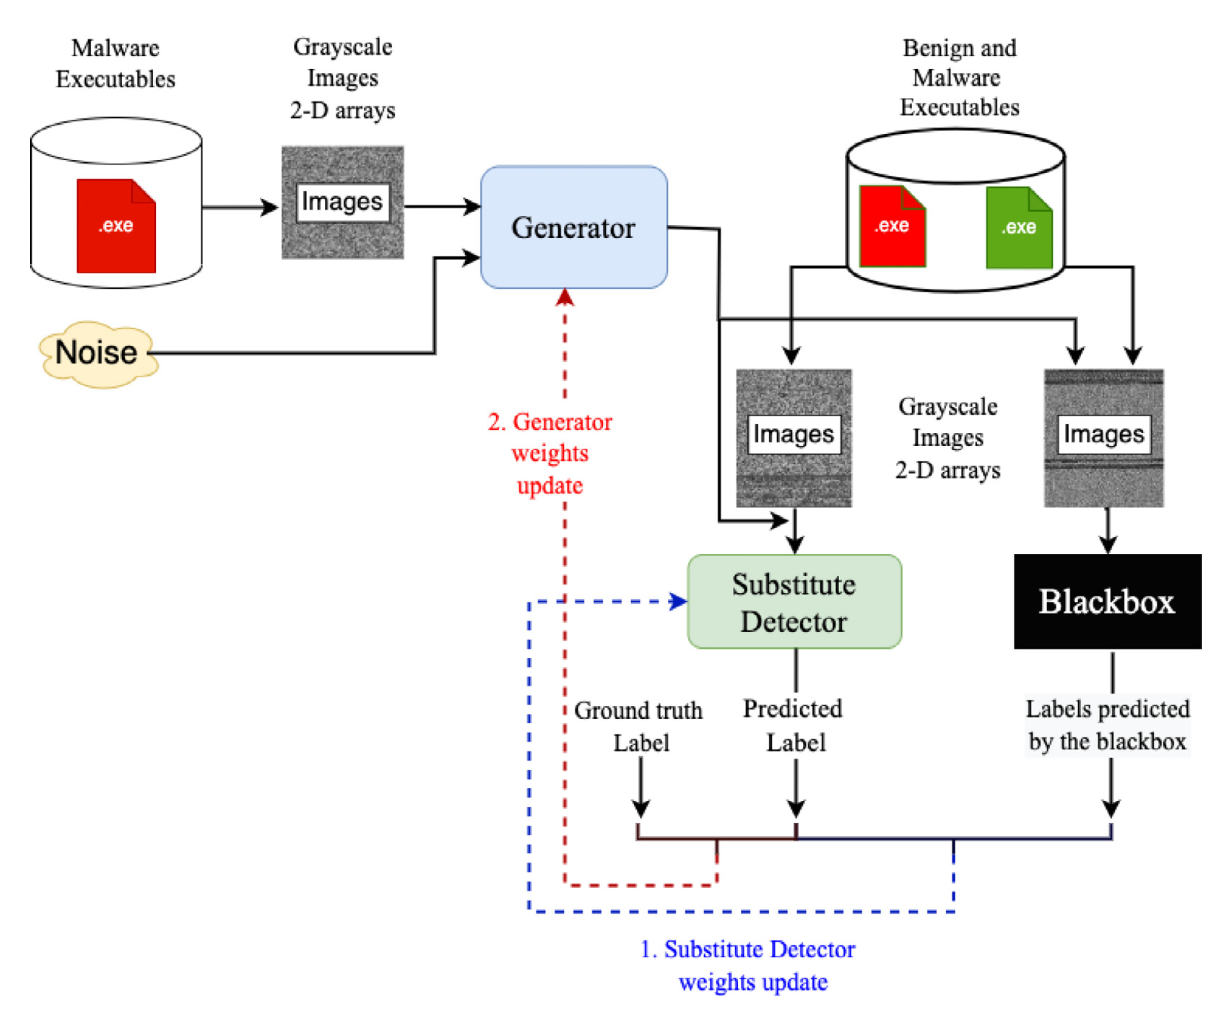
\includegraphics[width=0.6\linewidth]{images/GAN_architecture.png}
        \label{fig:gan_architecture}
        \caption{\emph{Architettura della Generative Adversarial Network (GAN) utilizzata}}
\end{figure}

\newpage

\subsubsection{Generatore}
\subsubsubsection{Struttura}
Il generatore è progettato per creare immagini realistiche aggiungendo rumore controllato a immagini reali. La sua struttura è composta da una sequenza di livelli densi, culminanti in una trasformazione che produce immagini con la stessa dimensione di quelle del dataset. L'architettura combina un input di rumore latente, etichette di classe e immagini reali, producendo immagini alterate attraverso l'operazione di somma.
\subsubsubsection{Funzionamento}
Il generatore opera applicando un rumore progressivo alle immagini reali, guidato da un vettore latente e dalle etichette di classe. Il rumore viene gradualmente adattato durante l'addestramento, ottimizzando il modello per produrre immagini che siano percepite come realistiche dal discriminatore (substitute detector). La perdita del generatore include una componente che misura l'inganno del modello \emph{blackbox} e una regolarizzazione basata sulla somiglianza con le immagini originali.
\subsubsubsection{Processo di addestramento}
Il generatore viene addestrato utilizzando gradienti calcolati sulla base della capacità di ingannare il modello ``blackbox''. Durante ogni epoca, il rumore viene progressivamente regolato in base a una funzione sigmoidea, incrementando il suo impatto sulle immagini. La loss del generatore viene ottimizzata minimizzando la distanza tra le immagini reali e generate, e massimizzando l'inganno del \gls{blackboxmodel}. Inoltre, le immagini generate vengono validate per assicurare che rispettino la distribuzione del dataset reale.

\begin{figure}[ht]
    \centering
        \centering
        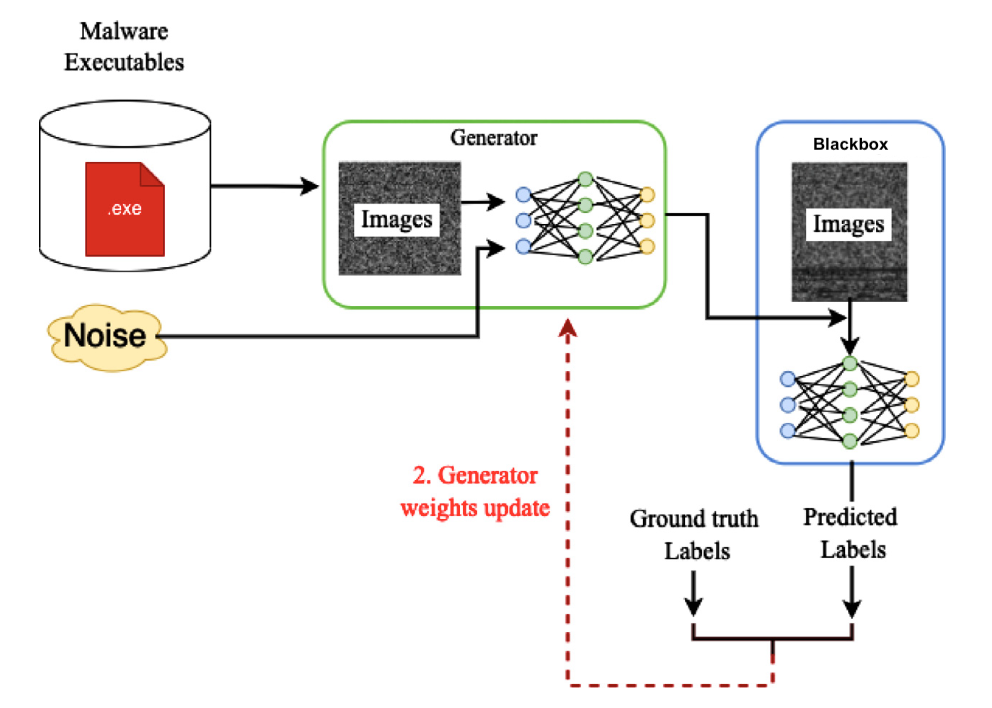
\includegraphics[width=0.6\linewidth]{images/generator_training.png}
        \caption{\emph{Processo di addestramento del Generatore}}
        \label{fig:generator_train}
\end{figure}

\newpage

\subsubsection{Discriminatore}
\subsubsubsection{Struttura}
Il discriminatore, chiamato anche \emph{substitute detector}, è un modello convoluzionale progettato per classificare le immagini. La sua struttura include strati convoluzionali per estrarre caratteristiche rilevanti, seguiti da uno strato di pooling e da livelli densi per la classificazione finale. L'output è una distribuzione di probabilità sulle classi del dataset.

\subsubsubsection{Funzionamento}
Il discriminatore riceve sia immagini reali che generate come input e tenta di classificarle in base alle classi del dataset. Il modello è ottimizzato per distinguere accuratamente tra immagini appartenenti a classi diverse, fornendo un feedback cruciale al generatore durante l'addestramento.

\subsubsubsection{Processo di addestramento}
Il discriminatore viene addestrato simultaneamente al generatore, utilizzando immagini reali e generate. La sua funzione di perdita è la cross-entropy categoriale, calcolata sulle etichette reali e le predizioni del modello. Durante il processo, i gradienti vengono propagati per affinare i pesi del discriminatore, migliorandone la capacità di classificazione. Le prestazioni vengono monitorate utilizzando metriche di accuratezza, precisione, richiamo e F1-score sia sulle immagini di training che di validazione.

\begin{figure}[ht]
    \centering
        \centering
        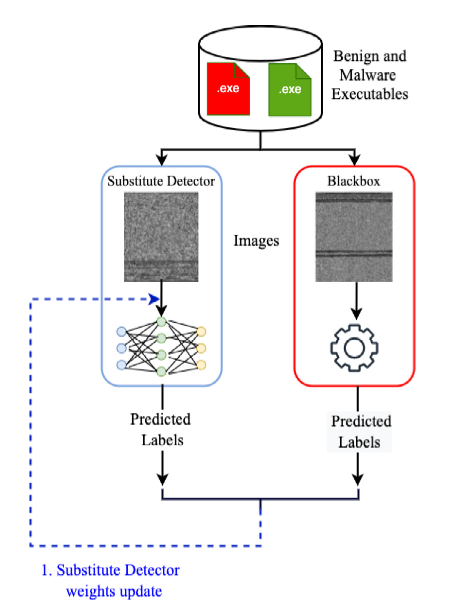
\includegraphics[width=0.5\linewidth]{images/discriminator_train.png}
        \caption{\emph{Processo di addestramento del Substitute Detector}}
        \label{fig:discriminator_train}
\end{figure}

\newpage

\subsubsection{Blackbox}
Il modello \emph{Blackbox} rappresenta un sistema di classificazione pre-addestrato, utilizzato come riferimento durante il processo di addestramento del generatore e del discriminatore. Questo modello è responsabile della classificazione delle immagini generate, fornendo un feedback critico per valutare l'efficacia del generatore nel creare immagini che ingannino il classificatore. Il blackbox funge quindi da obiettivo principale del generatore, il quale cerca di massimizzare la confusione del modello attraverso l'ottimizzazione delle sue uscite.


\subsubsection{Applicazioni}
Le Generative Adversarial Networks rappresentano una delle architetture di machine learning più innovative e potenti degli ultimi anni. Combinando due reti neurali, il generatore e il discriminatore, le GAN sono state applicate con successo in numerosi ambiti, tra cui la generazione di immagini, la sintesi del linguaggio e, più recentemente, nella rilevazione e creazione di malware. Sebbene le GAN siano principalmente note per la loro capacità di generare dati sintetici altamente realistici, il loro impiego in cybersecurity, e in particolare nella manipolazione e generazione di malware, sta acquisendo sempre più attenzione.

\subsubsubsection{Generazione di Malware per l'Analisi e la Rilevazione}
Una delle applicazioni emergenti delle GAN nel contesto del malware è la generazione di malware sintetico. Le GAN possono essere utilizzate per creare nuovi campioni di malware che replicano le caratteristiche delle minacce informatiche esistenti. Questo approccio consente di arricchire i dataset di malware, che sono spesso sbilanciati o insufficienti, con nuovi esempi che possono essere utilizzati per addestrare modelli di rilevazione più robusti e accurati. Generando malware sintetico, è possibile simulare scenari di attacco reali senza compromettere la sicurezza, permettendo agli esperti di cybersecurity di testare e affinare i sistemi di difesa.
Le GAN si distinguono particolarmente nella creazione di varianti di malware che mantengono le stesse caratteristiche funzionali ma con differenze sufficienti da eludere i sistemi di rilevamento tradizionali. Questi modelli generativi sono in grado di apprendere le modalità di evasione dei rilevatori, come quelli basati su firma o comportamentali, e creare malware che possiede capacità di auto-modifica, mimetizzandosi meglio nei sistemi di sicurezza.

\subsubsubsection{Miglioramento dei Sistemi di Rilevamento}
Un'altra area cruciale in cui le GAN stanno trovando applicazione è nel miglioramento dei sistemi di rilevamento del malware. Tradizionalmente, i sistemi di rilevamento si basano su tecniche come l'analisi delle firme o l'analisi comportamentale. Tuttavia, queste tecniche spesso falliscono quando il malware si evolve rapidamente, specialmente nei casi in cui il codice cambia per sfuggire ai sistemi di sicurezza. Le GAN, in questo caso, possono essere utilizzate per addestrare modelli di rilevamento più robusti, generando nuovi campioni di malware che i sistemi di difesa non hanno mai visto prima.
L'approccio di adversarial training (addestramento avversario) con le GAN è particolarmente promettente: durante l'addestramento, il generatore crea malware sintetico che viene utilizzato per ingannare il discriminatore, che cerca di classificarlo come malware o come software legittimo. Questo processo aiuta a migliorare la capacità del modello di rilevare anche minacce sconosciute e mai viste, aumentando l'efficacia dei sistemi di sicurezza.

\subsubsubsection{Evasione e Attacchi Avanzati}
Le GAN sono anche utilizzate in ambito offensivo per creare attacchi adversariali mirati, cioè malware progettato per aggirare specifici sistemi di difesa. Utilizzando la capacità delle GAN di generare nuovi dati in modo iterativo e migliorato, gli attaccanti possono creare malware che riesce a bypassare i sistemi di rilevazione basati su machine learning. In questo caso, il generatore produce varianti del malware che cercano deliberatamente di eludere i filtri di rilevamento, mentre il discriminatore aiuta a ottimizzare il processo di evasione, rendendo l'attacco sempre più difficile da identificare.

\subsubsection{Tipologie}
Esistono numerosi tipi e varianti di GAN, progettati per migliorare le prestazioni in compiti specifici come la generazione di immagini, il miglioramento della qualità delle immagini, o l'adattamento ai dati di input. Di seguito vengono descritti alcuni dei modelli più rilevanti e simili al modello sviluppato durante il periodo di tirocinio: MiGAN, MalGAN, Xception, e InceptionNet.

\subsubsubsection{MiGAN (Malware Image Generative Adversarial Network)}
MiGAN è una variante delle GAN utilizzata per la generazione di immagini di malware. È particolarmente utile nel campo della cybersecurity per migliorare la rilevazione e la generazione di nuove varianti di malware, e si concentra sulla sintesi di immagini di malware che imitano le caratteristiche visive delle minacce esistenti ma con l'intento di eludere i sistemi di rilevamento.

\subsubsubsubsection{Architettura di MiGAN}
L'architettura di MiGAN è composta da un generatore e da un discriminatore, simile a una GAN tradizionale, ma progettata per gestire immagini di malware. La struttura del modello è la seguente:
\begin{itemize}
    \item \textbf{Generatore (G)}: Il generatore crea immagini di malware sintetiche a partire da un vettore di rumore casuale, utilizzando convoluzioni trasposte e batch normalization. La rete è composta da diversi strati di convoluzione, ognuno dei quali espande la dimensione dell'immagine, partendo da un basso livello di dettaglio a uno più alto. 
    \begin{itemize}
        \item Strato di \texttt{Dense}: Per iniziare con un vettore di rumore.
        \item Strato \texttt{Reshape}: Per adattare l'output del \texttt{Dense} in una forma adatta alla convoluzione.
        \item Strati di \texttt{Conv2DTranspose}: Convoluzioni trasposte per ingrandire l'immagine.
        \item \texttt{BatchNormalization}: Per migliorare la stabilità dell'apprendimento.
        \item Funzione di attivazione \texttt{ReLU}: Per la maggior parte degli strati.
        \item \texttt{Tanh}: Per l'output, che restituisce valori tra -1 e 1, tipici delle immagini.
    \end{itemize}
    \item \textbf{Discriminatore (D)}: Il discriminatore è una rete neurale convoluzionale che cerca di distinguere tra immagini di malware reali e quelle sintetiche. Essa utilizza convoluzioni per ridurre progressivamente la dimensione spaziale dell'immagine, utilizzando anche \texttt{LeakyReLU} come funzione di attivazione.
    \begin{itemize}
        \item Strati \texttt{Conv2D}: Convoluzioni per l'estrazione delle caratteristiche.
        \item \texttt{LeakyReLU}: Per prevenire i vanishing gradients.
        \item \texttt{Dropout}: Per evitare overfitting.
        \item \texttt{Flatten}: Per appiattire l'immagine.
        \item \texttt{Dense}: Per ottenere una singola probabilità tra 0 (reale) e 1 (falsa).
    \end{itemize}
\end{itemize}
Questa architettura consente di generare nuove varianti di malware che possono essere utilizzate per allenare modelli di rilevamento più robusti.

\subsubsubsection{MalGAN (Malware Generative Adversarial Network)}
MalGAN è un'architettura GAN progettata per eludere i sistemi di rilevamento del malware esistenti. A differenza di MiGAN, che genera immagini di malware, MalGAN si concentra sulla creazione di varianti che possano bypassare i modelli di machine learning tradizionali.
\subsubsubsubsection{Architettura di MalGAN}
MalGAN si basa su un'architettura GAN simile a quella di MiGAN, ma con un focus sull'ottimizzazione delle capacità di evasione. In particolare, MalGAN integra un meccanismo di \textit{adversarial training} per creare esempi di malware che sono difficili da rilevare dai modelli di sicurezza.
\begin{itemize}
    \item \textbf{Generatore (G)}: Crea varianti di malware per ingannare il discriminatore. Il generatore è composto da:
    \begin{itemize}
        \item Strato \texttt{Dense} seguito da \texttt{Reshape}.
        \item Strati \texttt{Conv2DTranspose} per amplificare la dimensione dell'immagine.
        \item Normalizzazione e \texttt{ReLU} per attivazioni.
    \end{itemize}
    \item \textbf{Discriminatore (D)}: È un classificatore binario che distingue tra malware reale e generato. Utilizza:
    \begin{itemize}
        \item Strati \texttt{Conv2D} con \texttt{LeakyReLU}.
        \item \texttt{Dropout} per migliorare la generalizzazione.
        \item Funzione di attivazione \texttt{Sigmoid} per la probabilità di autenticità.
    \end{itemize}
\end{itemize}
Il modello di MalGAN è addestrato su varianti di malware esistenti, cercando di ottimizzare la sua capacità di generare malware che può sfuggire ai rilevatori.

\subsubsubsection{Xception (Extreme Inception)}
Xception è una rete neurale convoluzionale basata su una versione avanzata di Inception, ed è progettata per migliorare l'efficienza computazionale attraverso l'uso di convoluzioni separabili in profondità.
\subsubsubsubsection{Architettura di Xception}
Xception\cite{site:machinelearningtutorials} si distingue dall'architettura Inception tradizionale, poiché utilizza convoluzioni separabili in profondità, che separano le convoluzioni spaziali e di canale. Questo approccio migliora l'efficienza computazionale e consente una maggiore espressione del modello.
\begin{itemize}
    \item \textbf{Convoluzioni separabili in profondità}: Separano le operazioni di convoluzione in due passaggi: uno per ciascun canale e uno per la combinazione dei canali. Questo riduce il numero di parametri e aumenta l'efficienza.
    \item Strati \texttt{Conv2D}: Applicati ai dati separatamente per ciascun canale.
    \item Strati \texttt{MaxPooling2D}: Per ridurre le dimensioni spaziali.
    \item \texttt{GlobalAveragePooling2D}: Utilizzato per ridurre le dimensioni della feature map, migliorando la generalizzazione.
    \item Strati \texttt{Dense}: Per la classificazione finale con \texttt{Softmax}.
\end{itemize}
Questa architettura è ampiamente utilizzata in compiti di visione artificiale, inclusa la classificazione delle immagini.

\subsubsubsection{InceptionNet}
InceptionNet è una rete neurale convoluzionale progettata per essere altamente efficiente, utilizzando un approccio modulare che combina convoluzioni di diverse dimensioni e pooling.
\subsubsubsubsection{Architettura di InceptionNet}
InceptionNet utilizza moduli Inception che permettono di eseguire convoluzioni di diverse dimensioni, migliorando la capacità della rete di apprendere a più scale.
\begin{itemize}
    \item \textbf{Inception Module}: Ogni modulo esegue convoluzioni di diverse dimensioni (1x1, 3x3, 5x5) e le concatena, permettendo alla rete di esplorare diverse scale di caratteristiche.
    \item Strati \texttt{Conv2D}: Eseguiti con kernel di dimensioni diverse all'interno dello stesso modulo.
    \item \texttt{Pooling Layers}: Combinazione di max-pooling e average-pooling.
    \item \texttt{1x1 Convoluzioni}: Utilizzate per ridurre la dimensionalità, migliorando l'efficienza computazionale.
    \item Strati \texttt{Dense}: Per la classificazione finale.
    \item \texttt{Softmax}: Per la normalizzazione delle probabilità.
\end{itemize}
Questa architettura è stata utilizzata con successo in competizioni di riconoscimento delle immagini e classificazione di oggetti, come il ImageNet Challenge.

\section{Problematiche}
\label{Problema}
Durante lo svolgimento del progetto, sono state riscontrate diverse problematiche che hanno influenzato negativamente le prestazioni del modello e la sua efficienza nel rilevamento del malware. Le principali includono:
\begin{enumerate}
  \item \textbf{Squilibrio del dataset:} Il dataset era notevolmente sbilanciato, risultando in una riduzione della precisione e dell'accuratezza del modello. Questo squilibrio ha limitato la capacità del modello di rappresentare efficacemente tutte le classi di malware, compromettendo la sua abilità di generalizzare e rilevare nuove varianti di malware.
  \item \textbf{Dimensioni del dataset:} Le dimensioni ridotte del dataset hanno impedito una rappresentazione accurata e completa delle diverse classi di malware. Inoltre, la classificazione è stata effettuata per superfamiglie anziché per singole famiglie, il che ha ulteriormente ridotto la precisione e l'accuratezza del modello, poiché le superfamiglie aggregano molteplici classi con caratteristiche simili.
  \item \textbf{Architettura del modello:} L'architettura attuale del modello potrebbe beneficiare di miglioramenti. L'adozione di architetture più avanzate, come Xception o InceptionNet, potrebbe significativamente migliorare le prestazioni.
  \item \textbf{Limitazioni delle risorse hardware:} Le limitate capacità computazionali della macchina utilizzata per l'addestramento e i test hanno comportato tempi di addestramento prolungati e hanno ristretto la nostra capacità di esplorare a fondo l'architettura del modello e di ottimizzare i parametri.
\end{enumerate}
Queste limitazioni hanno evidenziato la necessità di un ulteriore sviluppo e ottimizzazione per superare queste sfide e migliorare l'efficacia del modello nel rilevamento del malware.


\subsection{Miglioramenti}
Di seguito sono riportati i principali miglioramenti proposti per affrontare le problematiche identificate e ottimizzare il modello di rilevamento del malware:
\begin{enumerate}
    \item \textbf{Miglioramento del Dataset}:
      \begin{itemize}
        \item \textbf{Bilanciamento}: Ridurre lo sbilanciamento nel dataset, rendendolo non solo più equilibrato ma anche più rappresentativo delle varie classi di malware.
        \item \textbf{Accuratezza e Dimensioni}: Espansione del dataset, rendendolo più grande e accurato, migliorando significativamente la qualità e l'affidabilità dei dati disponibili per l'addestramento del modello.
      \end{itemize}
  
    \item \textbf{Classificazione Raffinata}:
      \begin{itemize}
        \item \textbf{Per Famiglia e Superfamiglia}: Introduzione di una classificazione più dettagliata, sia per singole famiglie sia per superfamiglie di malware, aumenterebbe la precisione del modello nella rilevazione delle minacce, permettendo un' identificazione più specifica e accurata.
      \end{itemize}
  
    \item \textbf{Perfezionamento dell'Architettura del Modello}:
      \begin{itemize}
        \item \textbf{Miglioramento dei Layer}: Dedicare più tempo all'ottimizzazione della struttura dei layer permetterebbe una migliore elaborazione delle caratteristiche e un'apprendimento più efficace, portando di conseguenza ad un aumento delle prestazioni complessive del sistema.
      \end{itemize}

    \item \textbf{Utilizzo di Architetture Avanzate}:
      \begin{itemize}
        \item \textbf{Xception e InceptionNet}: L'adozione di architetture più avanzate e performanti, come Xception e InceptionNet, potrebbe migliorare significativamente le prestazioni del modello, consentendo una migliore rappresentazione delle caratteristiche e una maggiore capacità di generalizzazione.
      \end{itemize}
  \end{enumerate}
  
Questi avanzamenti renderebbero il modello non solo più robusto ma anche più efficiente nel rilevare e classificare vari tipi di malware con una maggiore precisione.
  